\chapter{AWS Deployment \\
\small{\textit{-- Nataly Jimenez, Nicole Valdiviezo, Lakshya Vegiraju}}
\index{AWS Deployment} 
\index{Chapter!AWS Deployment}
\label{Chapter::AWS Deployment}}

This chapter documents step-by-step how to deploy the Two Buttons website to AWS using ECR + App Runner. The color buttons application was successfully deployed to Amazon Web Services using ECR and ECS with Fargate.

\section{Verifying If AWS CLI Is Already Installed}

\begin{minted}{bash}
aws --version
# Returned: 
\end{minted}

\section{Post-Install Configuration and Confirming Credentials Are Working}
\begin{minted}{bash}
aws configure sso:
# Example answers:
# SSO session name: my-sso
# SSO start URL: https://YOUR-SUBDOMAIN.awsapps.com/start
# SSO region: us-east-2
# Account: <select>
# Role:
AdministratorAccess (or your role)
# Default region: us-east-2
# Output: json
# Login
aws sso login --profile default
aws configure# AWS Access Key ID: <AKIA...>
# AWS Secret Access Key: <...>
# Default region name: us-east-2
# Default output format: json
ws sts get-caller-identity
\end{minted}

\section{Create AWS Account}
1. Go to aws.amazon.com → Create an AWS Account.
2. Log in as the root user once to complete setup.
3. Enable MFA on the root account: AWS Console → IAM → Dashboard → Activate MFA on
your root account. Store recovery codes safely.
4. Choose a home region (e.g., us-east-2) and use it consistently in commands

\section{Set Cost Budget}
1. Console: Billing → Budgets → Create budget.
2. Budget type: Cost budget, amount e.g. \$10/month.
3. Configure alerts at 50\%, 80\%, and 100\% to your email.

\section{Enable IAM Identity Center (SSO)}
1. Console: IAM Identity Center → Enable.
2. Create a user for yourself (e.g., your work email)
3. Create or assign a Permission Set: start with AdministratorAccess. (You can later add a
least-privilege set for ECR push.)
4. Record your SSO Start URL (you’ll need it in the CLI).

\section{Install and Configure AWS CLI for SSO}

\begin{minted}{bash}
sudo apt-get update && sudo apt-get install -y unzip
curl "https://awscli.amazonaws.com/awscli-exe-linux-x86_64.zip" -o "awscliv2.zip"
unzip awscliv2.zip && sudo ./aws/install
aws configure sso# Prompts (example answers):
# SSO session name: my-sso
# SSO start URL: https://YOUR-SUBDOMAIN.awsapps.com/start
# SSO region: us-east-2
# Account: <select your new account>
# Role: AdministratorAccess
# Default region: us-east-2
# Output: json
# Log in via browser:
aws sso login --profile default
\end{minted}

\section{Set Environmental Variables}
\begin{minted}{bash}
# >>> EDIT THESE <<<
export AWS_REGION=us-east-1
export ECR_REPO=myapp
export IMAGE_TAG=v1
export CONTAINER_PORT=3000
# Port your app listens on
# Discover your AWS Account ID from your SSO session:
export AWS_ACCOUNT_ID="$(aws sts get-caller-identity --query Account --output text --profile default)"
\end{minted}

\section{Create an ECR Repo}
\begin{minted}{bash}
aws ecr describe-repositories \
--repository-names "$ECR_REPO" \
--region "$AWS_REGION" --profile default >/dev/null 2>&1 || \
aws ecr create-repository \
--repository-name "$ECR_REPO" \
--image-scanning-configuration scanOnPush=true \
--region "$AWS_REGION" --profile default
\end{minted}

\section{Authenticate Docker to ECR}
\begin{minted}{bash}
aws ecr get-login-password --region "$AWS_REGION" --profile default \
| docker login --username AWS --password-stdin \
"$AWS_ACCOUNT_ID.dkr.ecr.$AWS_REGION.amazonaws.com"
\end{minted}

\section{Build, Tag and Push Local Image}
\begin{minted}{bash}
docker build --platform linux/amd64 -t "$ECR_REPO:$IMAGE_TAG" .
# Tag it for ECR
docker tag "$ECR_REPO:$IMAGE_TAG" \
"$AWS_ACCOUNT_ID.dkr.ecr.$AWS_REGION.amazonaws.com/$ECR_REPO:$IMAGE_TAG"
# Push to ECR
docker push "$AWS_ACCOUNT_ID.dkr.ecr.$AWS_REGION.amazonaws.com/$ECR_REPO:$IMAGE_TAG"
\end{minted}

\section{Verify Image in ECR}
\begin{minted}{bash}
aws ecr describe-images \
--repository-name "$ECR_REPO" \
--region "$AWS_REGION" --profile default \
--query 'imageDetails[].imageTags'
\end{minted}


\section{Quick Deploy with App Runner}
\begin{minted}{bash}
export APP_NAME=my-apprunner-app
aws apprunner create-service \
--service-name "$APP_NAME" \
--region "$AWS_REGION" --profile default \
--source-configuration "{
\"ImageRepository\": {
\"ImageIdentifier\": \"$AWS_ACCOUNT_ID.dkr.ecr.$AWS_REGION.amazonaws.com/$ECR_REPO:$IMAGE_TAG\",
\"ImageRepositoryType\": \"ECR\",
\"ImageConfiguration\": {\"Port\": \"$CONTAINER_PORT\"}
},
\"AutoDeploymentsEnabled\": true
}" \
--instance-configuration "{\"Cpu\":\"1 vCPU\",\"Memory\":\"2 GB\"}"

AWS_REGION=us-east-2
PROFILE=AdministratorAccess-539272219501
SERVICE_ARN=arn:aws:apprunner:us-east-2:539272219501:service/my-apprunner-app/04c50b98cd0744369e395b654752a33c

while true; do
STATUS=$(aws apprunner describe-service \
--service-arn "$SERVICE_ARN" \
--region "$AWS_REGION" --profile "$PROFILE" \
--query 'Service.Status' --output text)
echo "Service status: $STATUS"
case "$STATUS" in RUNNING|CREATE_FAILED|OPERATION_FAILED) break ;; esac
sleep 4
done

aws apprunner list-services \
--region "$AWS_REGION" --profile default \
--query "ServiceSummaryList[?ServiceName=='$APP_NAME'].ServiceUrl" --output text
\end{minted}

\section{Security Checklist}
MFA enabled on the root account and your SSO user. Used SSO (no long-lived access keys on laptops). Cost budget with email alerts. Principle of least privilege for day-2 (created a minimal ECR Push permission set)

\section{AWS Website}
Links to AWS Website: 
\begin{verbatim}
    http://18.224.136.57:3000
\end{verbatim}
This is a dynamic public IP address assigned by AWS Fargate. The IP address will change if the task is stopped and restarted.

\section{AWS Account and Region Information}
\begin{itemize}
    \item UserId: AIDAZVOAA2MH4K2XESOC4
    \item AWS Acount ID: 664512025359
    \item Access Key: ****************ZGVP
    \item Region: us-east-2 (US East - Ohio)
    \item IAM User: ncvald
\end{itemize}

\section{ECS Deployment Information}

\begin{itemize}
    \item Cluster Name: my-cluster1
    \item Task Definition: color-buttons-task
    \item Service Type: AWS Fargate
    \item Container Port: 3000
\end{itemize}
\section{ECR Repository Information}
\begin{itemize}
    \item ECR Repository Name: color-button-app
    \item ECR Repository URI: 664512025359.dkr.ecr.us-east-2.amazonaws.com/color-button-app
    \item Image Tags: v1 (original), v2 (class-based JavaScript)
\end{itemize}

\section{Deployment Versions}
\begin{itemize}
    \item Version 1 (v1): Original implementation with function-based JavaScript.
    \\ Image URI: 664512025359.dkr.ecr.us-east-2.amazonaws.com/color-button-app:v1
    \item Version 2 (v2): Updated implementation with class-based JavaScript (current)
    \\Image URI: 664512025359.dkr.ecr.us-east-2.amazonaws.com/color-button-app:v2
    
\end{itemize}

\section{Images}

Below are images showing the color button app, the ECS task showing a RUNNING status, and the task details page showing the public IP
\begin{figure}
    \centering
    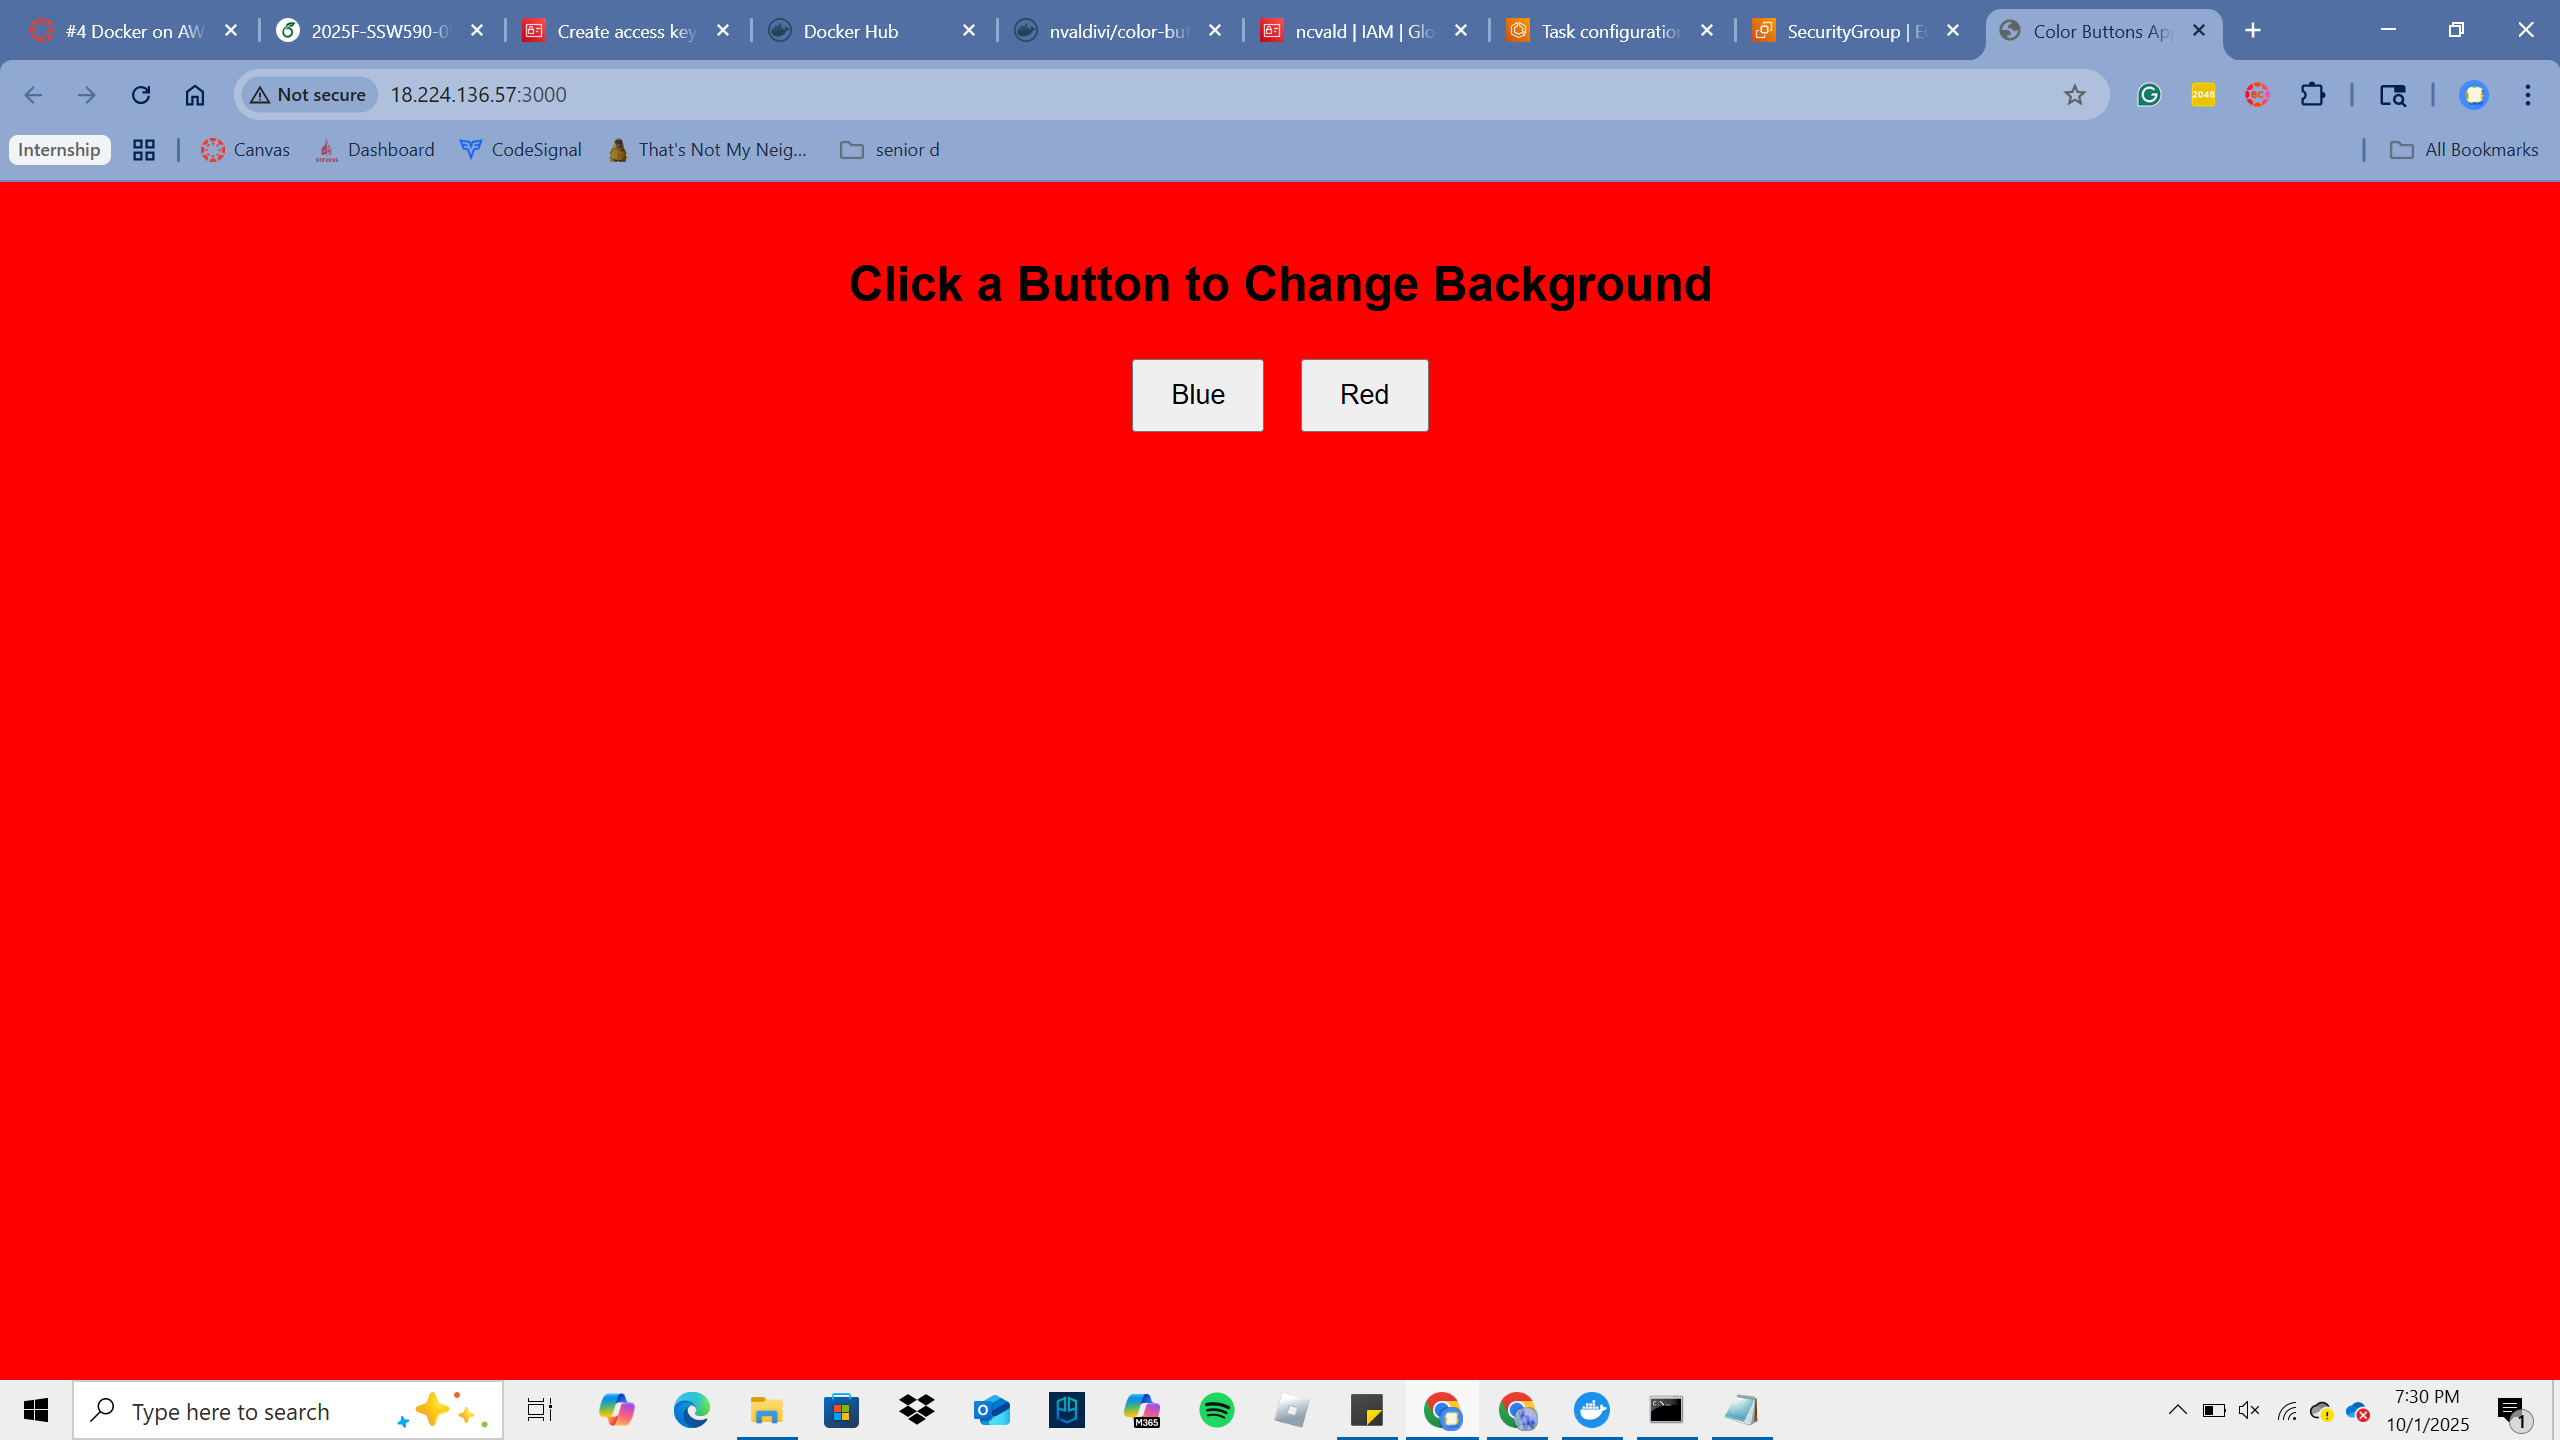
\includegraphics[width=0.6\linewidth]{Book_SSW590 (1)/eps/Screenshots/NewColorButton.png}
    \caption{Color Buttom App V2}
    \label{fig:Color Buttom App V2}
\end{figure}

\begin{figure}
    \centering
    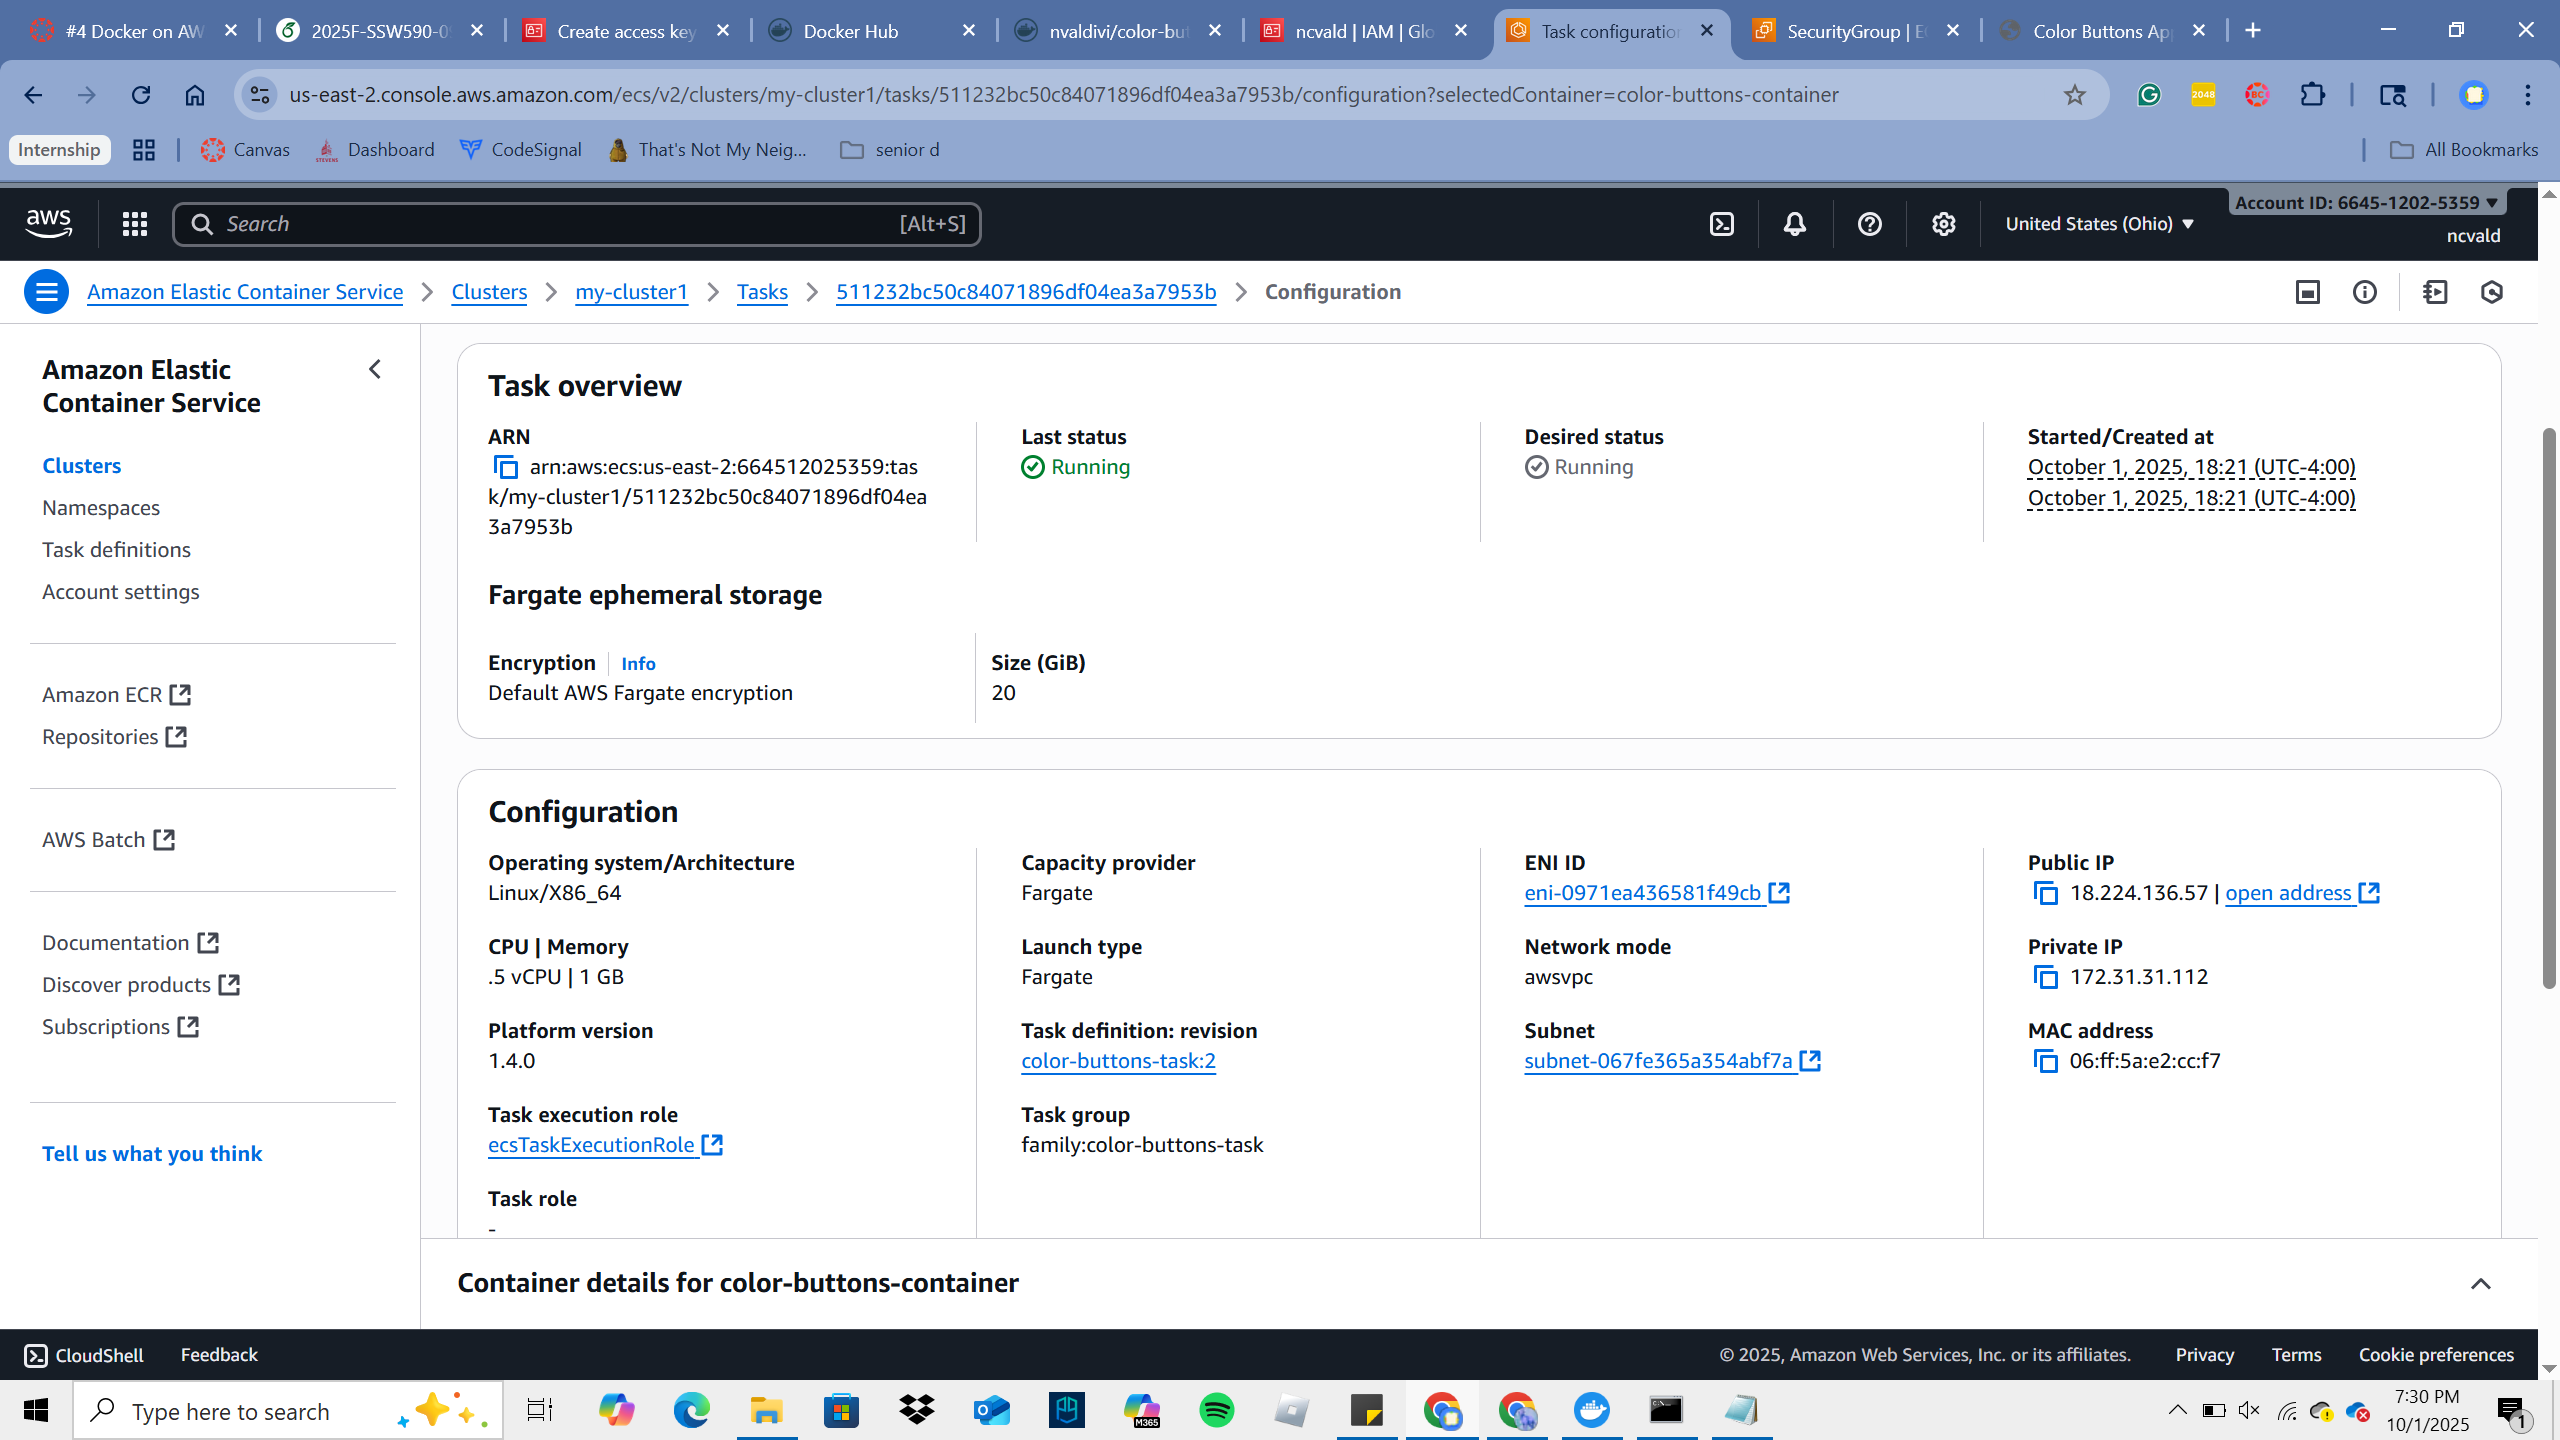
\includegraphics[width=0.6\linewidth]{Book_SSW590 (1)/eps/Screenshots/PublicIP.png}
    \caption{Public IP}
    \label{fig:Public IP}
\end{figure}

\begin{figure}
    \centering
    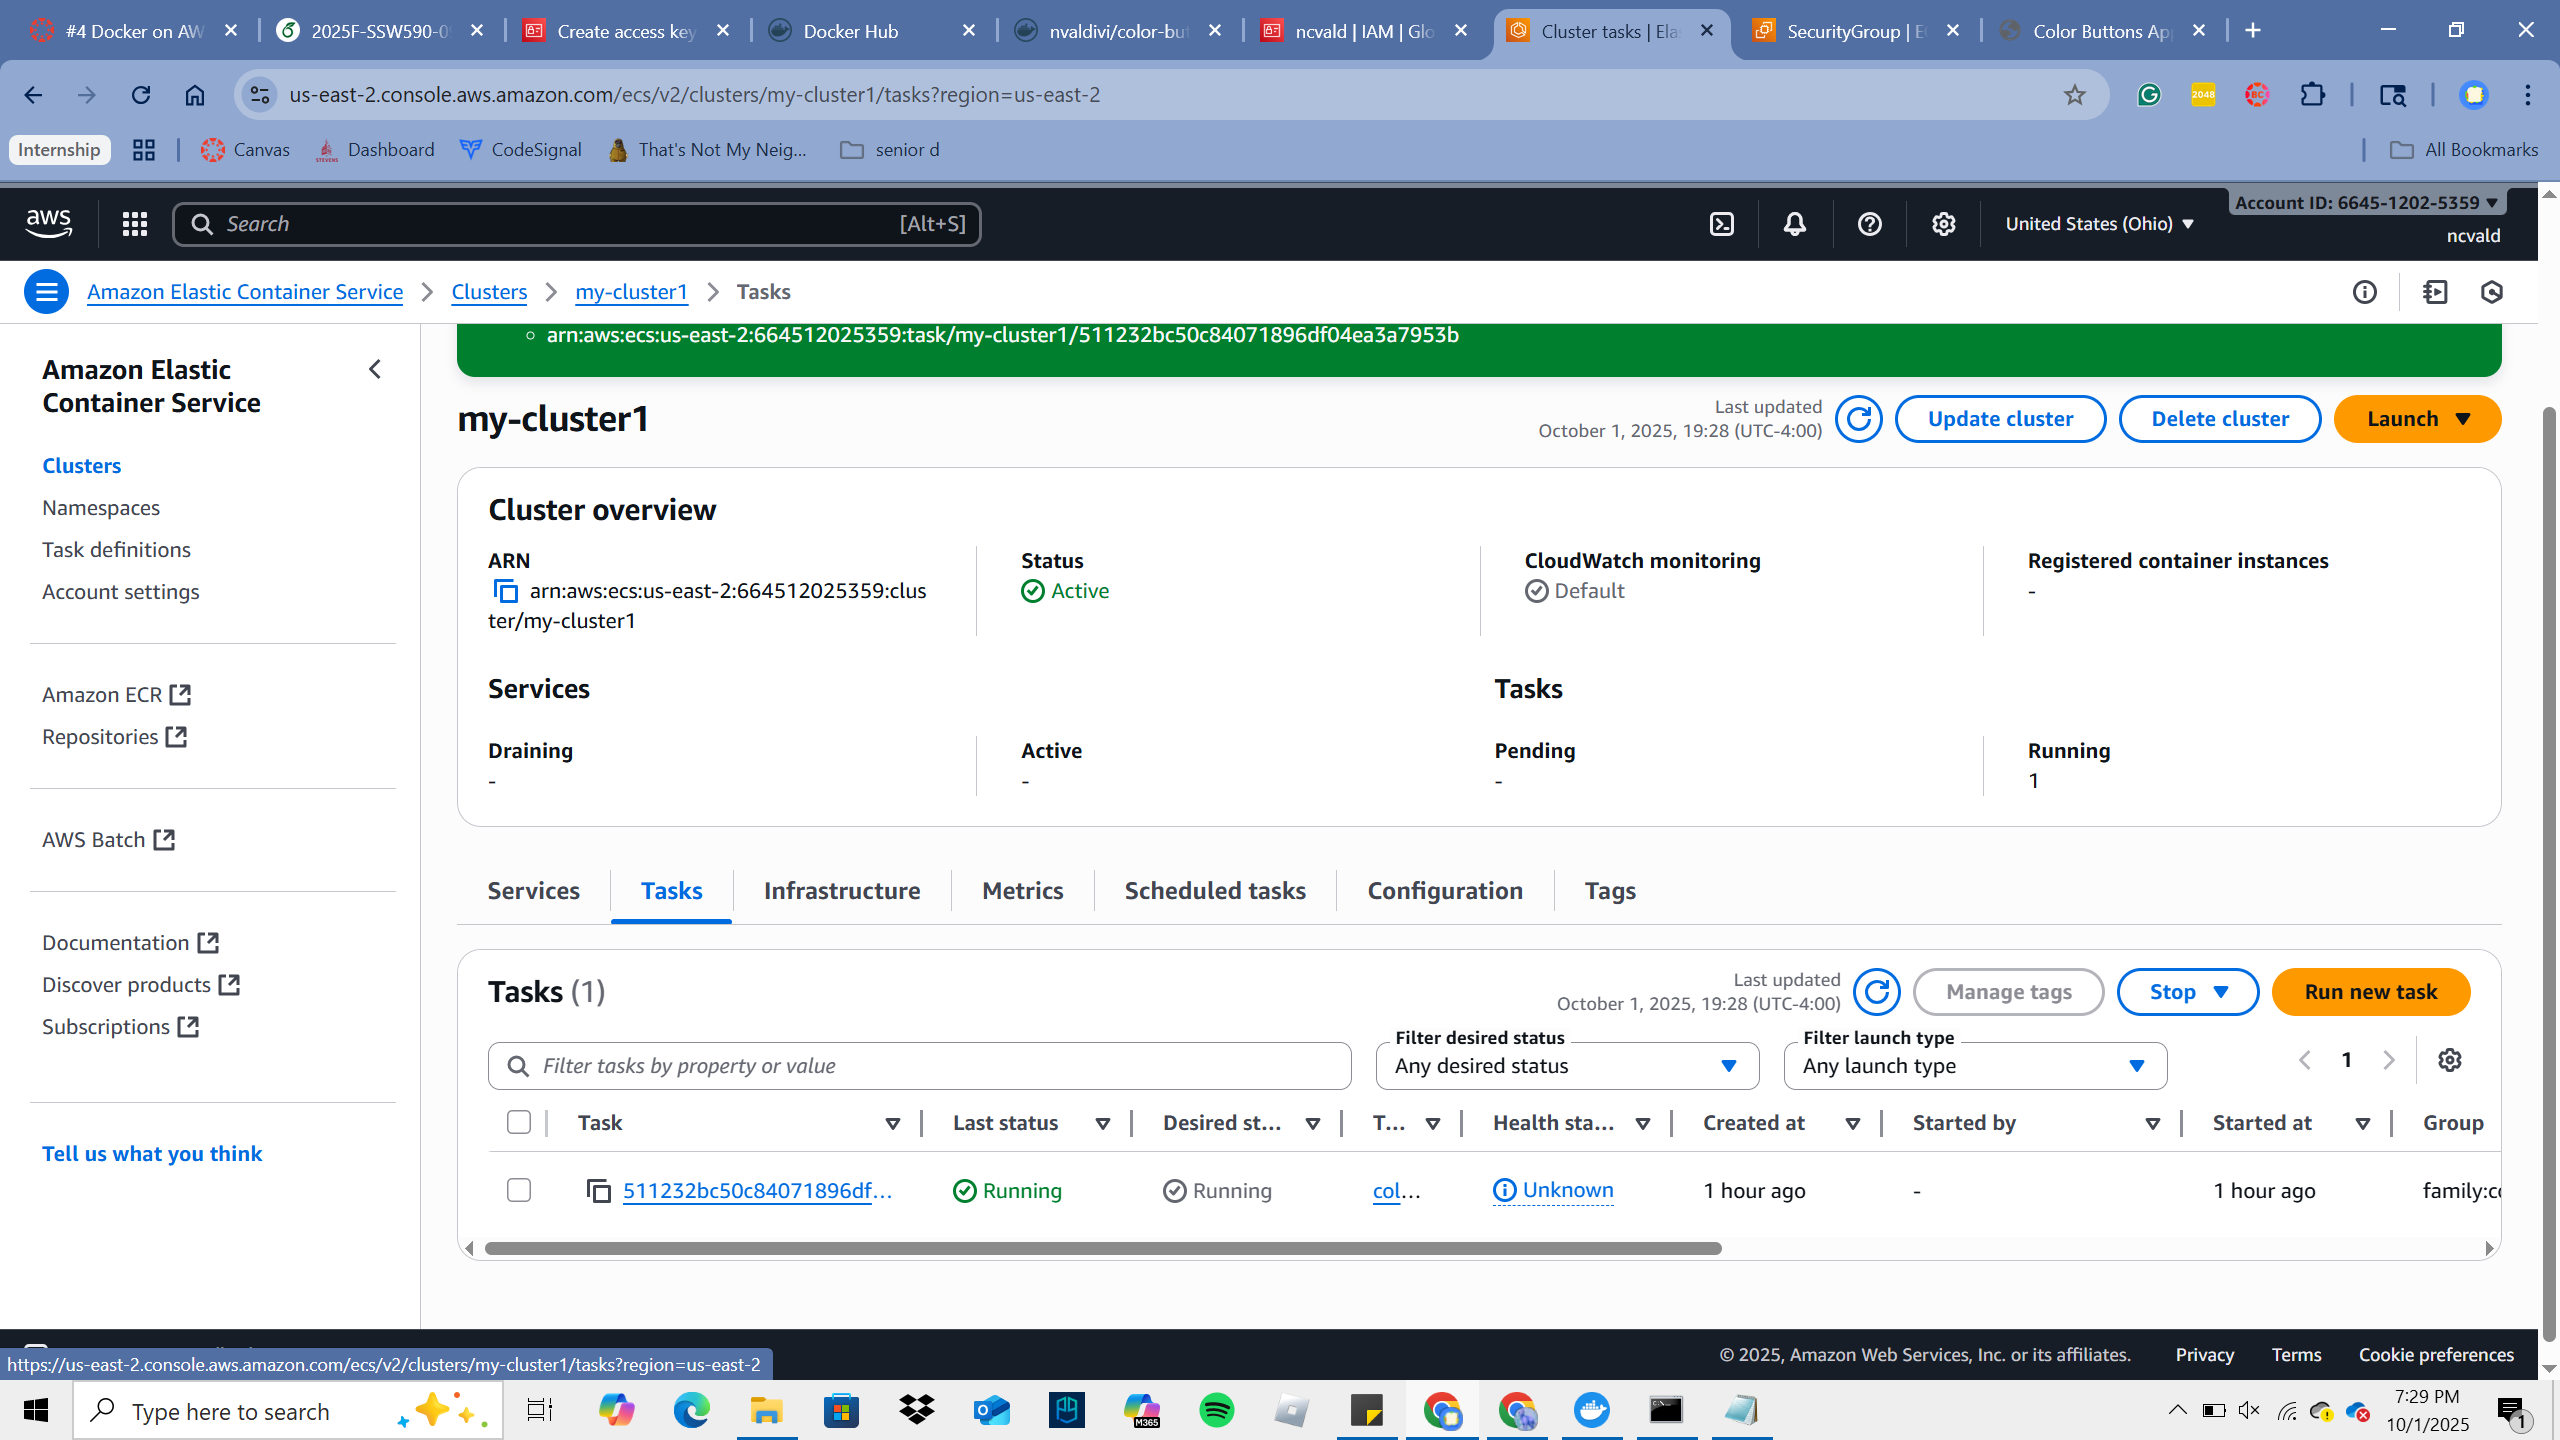
\includegraphics[width=0.6\linewidth]{Book_SSW590 (1)/eps/Screenshots/TaskRunning.png}
    \caption{Task Running}
    \label{fig:Tasking Running}
\end{figure}

\section{UML Class Design}
Below is an image of the UML class diagram for the updated design: changing the website for the two buttons to use a class-based javascript instead of methods: 

\begin{figure}[htbp]
\centering
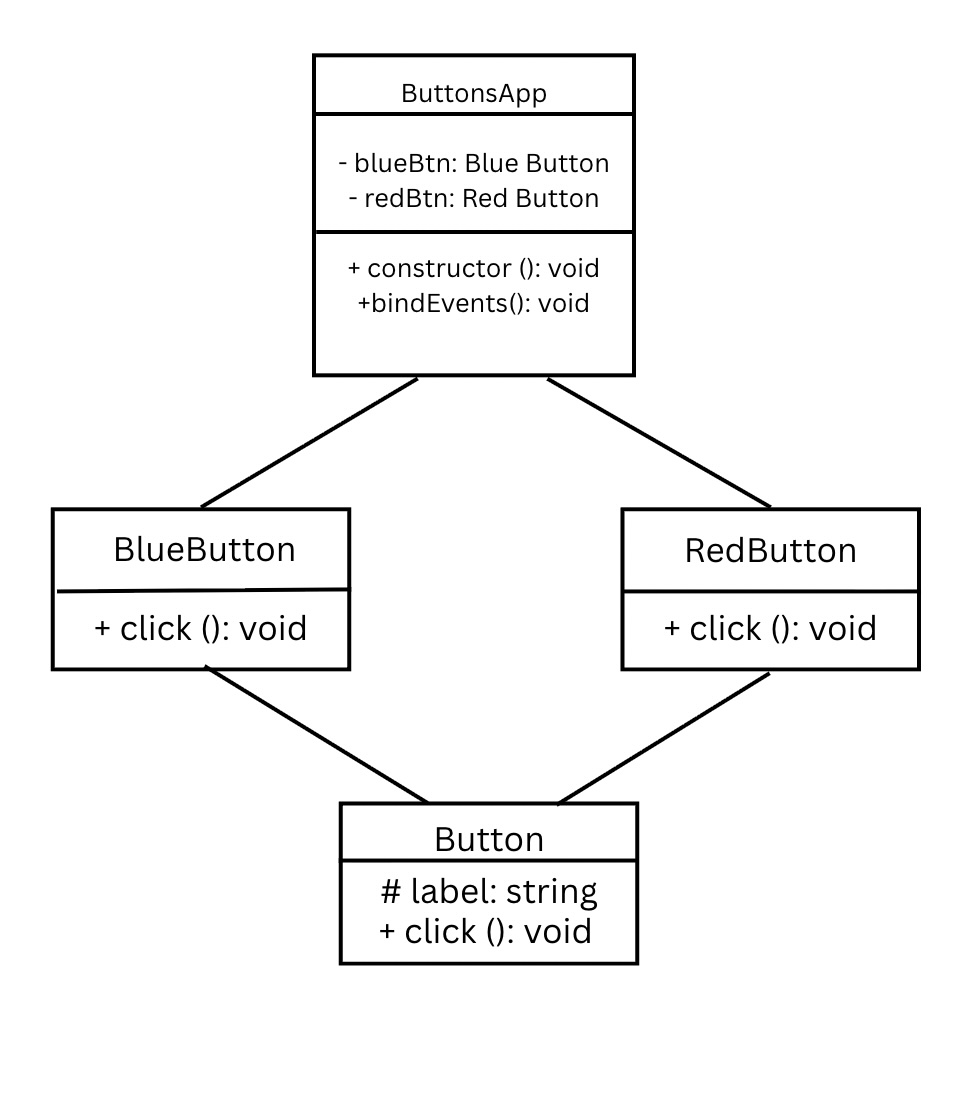
\includegraphics[width=0.85\linewidth]{uml_diagram.jpg}
\caption{UML class diagram for the class-based two-buttons app}
\label{fig:uml-diagram}
\end{figure}